% This file was created by matplotlib2tikz v0.7.4.
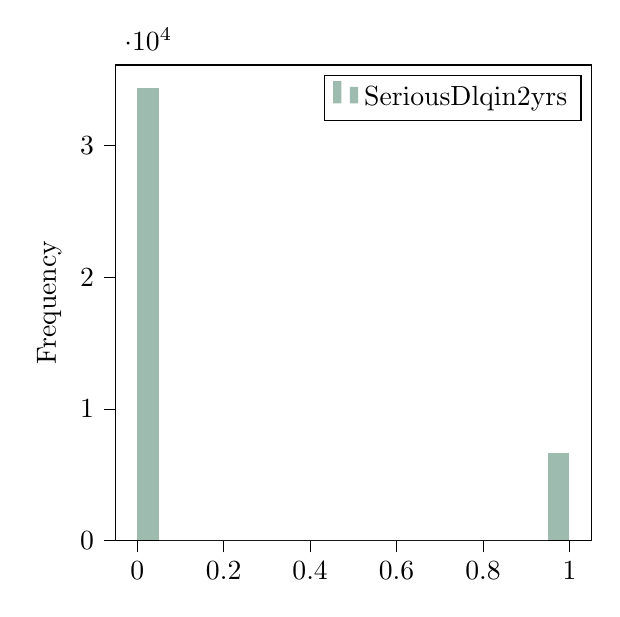
\begin{tikzpicture}

\definecolor{color0}{rgb}{0.615686274509804,0.733333333333333,0.682352941176471}

\begin{axis}[
height=3in,
tick align=outside,
tick pos=left,
width=3in,
x grid style={white!69.01960784313725!black},
xmin=-0.05, xmax=1.05,
xtick style={color=black},
y grid style={white!69.01960784313725!black},
ylabel={Frequency},
ymin=0, ymax=36115.8,
ytick style={color=black}
]
\draw[fill=color0,draw opacity=0] (axis cs:0,0) rectangle (axis cs:0.05,34396);
\addlegendimage{ybar,ybar legend,fill=color0,draw opacity=0};
\addlegendentry{SeriousDlqin2yrs}

\draw[fill=color0,draw opacity=0] (axis cs:0.05,0) rectangle (axis cs:0.1,0);
\draw[fill=color0,draw opacity=0] (axis cs:0.1,0) rectangle (axis cs:0.15,0);
\draw[fill=color0,draw opacity=0] (axis cs:0.15,0) rectangle (axis cs:0.2,0);
\draw[fill=color0,draw opacity=0] (axis cs:0.2,0) rectangle (axis cs:0.25,0);
\draw[fill=color0,draw opacity=0] (axis cs:0.25,0) rectangle (axis cs:0.3,0);
\draw[fill=color0,draw opacity=0] (axis cs:0.3,0) rectangle (axis cs:0.35,0);
\draw[fill=color0,draw opacity=0] (axis cs:0.35,0) rectangle (axis cs:0.4,0);
\draw[fill=color0,draw opacity=0] (axis cs:0.4,0) rectangle (axis cs:0.45,0);
\draw[fill=color0,draw opacity=0] (axis cs:0.45,0) rectangle (axis cs:0.5,0);
\draw[fill=color0,draw opacity=0] (axis cs:0.5,0) rectangle (axis cs:0.55,0);
\draw[fill=color0,draw opacity=0] (axis cs:0.55,0) rectangle (axis cs:0.6,0);
\draw[fill=color0,draw opacity=0] (axis cs:0.6,0) rectangle (axis cs:0.65,0);
\draw[fill=color0,draw opacity=0] (axis cs:0.65,0) rectangle (axis cs:0.7,0);
\draw[fill=color0,draw opacity=0] (axis cs:0.7,0) rectangle (axis cs:0.75,0);
\draw[fill=color0,draw opacity=0] (axis cs:0.75,0) rectangle (axis cs:0.8,0);
\draw[fill=color0,draw opacity=0] (axis cs:0.8,0) rectangle (axis cs:0.85,0);
\draw[fill=color0,draw opacity=0] (axis cs:0.85,0) rectangle (axis cs:0.9,0);
\draw[fill=color0,draw opacity=0] (axis cs:0.9,0) rectangle (axis cs:0.95,0);
\draw[fill=color0,draw opacity=0] (axis cs:0.95,0) rectangle (axis cs:1,6620);
\end{axis}

\end{tikzpicture}